
%% bare_adv.tex
%% V1.4a
%% 2014/09/17
%% by Michael Shell
%% See: 
%% http://www.michaelshell.org/
%% for current contact information.
%%
%% This is a skeleton file demonstrating the advanced use of IEEEtran.cls
%% (requires IEEEtran.cls version 1.8a or later) with an IEEE Computer
%% Society journal paper.
%%
%% Support sites:
%% http://www.michaelshell.org/tex/ieeetran/
%% http://www.ctan.org/tex-archive/macros/latex/contrib/IEEEtran/
%% and
%% http://www.ieee.org/

%%*************************************************************************
%% Legal Notice:
%% This code is offered as-is without any warranty either expressed or
%% implied; without even the implied warranty of MERCHANTABILITY or
%% FITNESS FOR A PARTICULAR PURPOSE! 
%% User assumes all risk.
%% In no event shall IEEE or any contributor to this code be liable for
%% any damages or losses, including, but not limited to, incidental,
%% consequential, or any other damages, resulting from the use or misuse
%% of any information contained here.
%%
%% All comments are the opinions of their respective authors and are not
%% necessarily endorsed by the IEEE.
%%
%% This work is distributed under the LaTeX Project Public License (LPPL)
%% ( http://www.latex-project.org/ ) version 1.3, and may be freely used,
%% distributed and modified. A copy of the LPPL, version 1.3, is included
%% in the base LaTeX documentation of all distributions of LaTeX released
%% 2003/12/01 or later.
%% Retain all contribution notices and credits.
%% ** Modified files should be clearly indicated as such, including  **
%% ** renaming them and changing author support contact information. **
%%
%% File list of work: IEEEtran.cls, IEEEtran_HOWTO.pdf, bare_adv.tex,
%%                    bare_conf.tex, bare_jrnl.tex, bare_conf_compsoc.tex,
%%                    bare_jrnl_compsoc.tex, bare_jrnl_transmag.tex
%%*************************************************************************


% *** Authors should verify (and, if needed, correct) their LaTeX system  ***
% *** with the testflow diagnostic prior to trusting their LaTeX platform ***
% *** with production work. IEEE's font choices and paper sizes can       ***
% *** trigger bugs that do not appear when using other class files.       ***                          ***
% The testflow support page is at:
% http://www.michaelshell.org/tex/testflow/


% IEEEtran V1.7 and later provides for these CLASSINPUT macros to allow the
% user to reprogram some IEEEtran.cls defaults if needed. These settings
% override the internal defaults of IEEEtran.cls regardless of which class
% options are used. Do not use these unless you have good reason to do so as
% they can result in nonIEEE compliant documents. User beware. ;)
%
%\newcommand{\CLASSINPUTbaselinestretch}{1.0} % baselinestretch
%\newcommand{\CLASSINPUTinnersidemargin}{1in} % inner side margin
%\newcommand{\CLASSINPUToutersidemargin}{1in} % outer side margin
%\newcommand{\CLASSINPUTtoptextmargin}{1in}   % top text margin
%\newcommand{\CLASSINPUTbottomtextmargin}{1in}% bottom text margin




%
\documentclass[10pt,journal,compsoc]{IEEEtran}
% If IEEEtran.cls has not been installed into the LaTeX system files,
% manually specify the path to it like:
% \documentclass[10pt,journal,compsoc]{../sty/IEEEtran}


% For Computer Society journals, IEEEtran defaults to the use of 
% Palatino/Palladio as is done in IEEE Computer Society journals.
% To go back to Times Roman, you can use this code:
%\renewcommand{\rmdefault}{ptm}\selectfont





% Some very useful LaTeX packages include:
% (uncomment the ones you want to load)



% *** MISC UTILITY PACKAGES ***
%
%\usepackage{ifpdf}
% Heiko Oberdiek's ifpdf.sty is very useful if you need conditional
% compilation based on whether the output is pdf or dvi.
% usage:
% \ifpdf
%   % pdf code
% \else
%   % dvi code
% \fi
% The latest version of ifpdf.sty can be obtained from:
% http://www.ctan.org/tex-archive/macros/latex/contrib/oberdiek/
% Also, note that IEEEtran.cls V1.7 and later provides a builtin
% \ifCLASSINFOpdf conditional that works the same way.
% When switching from latex to pdflatex and vice-versa, the compiler may
% have to be run twice to clear warning/error messages.






% *** CITATION PACKAGES ***
%
\ifCLASSOPTIONcompsoc
  % IEEE Computer Society needs nocompress option
  % requires cite.sty v4.0 or later (November 2003)
  \usepackage[nocompress]{cite}
\else
  % normal IEEE
  \usepackage{cite}
\fi
% cite.sty was written by Donald Arseneau
% V1.6 and later of IEEEtran pre-defines the format of the cite.sty package
% \cite{} output to follow that of IEEE. Loading the cite package will
% result in citation numbers being automatically sorted and properly
% "compressed/ranged". e.g., [1], [9], [2], [7], [5], [6] without using
% cite.sty will become [1], [2], [5]--[7], [9] using cite.sty. cite.sty's
% \cite will automatically add leading space, if needed. Use cite.sty's
% noadjust option (cite.sty V3.8 and later) if you want to turn this off
% such as if a citation ever needs to be enclosed in parenthesis.
% cite.sty is already installed on most LaTeX systems. Be sure and use
% version 5.0 (2009-03-20) and later if using hyperref.sty.
% The latest version can be obtained at:
% http://www.ctan.org/tex-archive/macros/latex/contrib/cite/
% The documentation is contained in the cite.sty file itself.
%
% Note that some packages require special options to format as the Computer
% Society requires. In particular, Computer Society  papers do not use
% compressed citation ranges as is done in typical IEEE papers
% (e.g., [1]-[4]). Instead, they list every citation separately in order
% (e.g., [1], [2], [3], [4]). To get the latter we need to load the cite
% package with the nocompress option which is supported by cite.sty v4.0
% and later.





% *** GRAPHICS RELATED PACKAGES ***
%
\ifCLASSINFOpdf
  \usepackage[pdftex]{graphicx}
  \usepackage[colorinlistoftodos]{todonotes}
  % declare the path(s) where your graphic files are
  \graphicspath{{content/img/}{content/img/}}
  % and their extensions so you won't have to specify these with
  % every instance of \includegraphics
  \DeclareGraphicsExtensions{.pdf,.jpg,.jpeg,.png,.PDF,.JPEG,.PNG}
\else
  % or other class option (dvipsone, dvipdf, if not using dvips). graphicx
  % will default to the driver specified in the system graphics.cfg if no
  % driver is specified.
  \usepackage[dvips]{graphicx}
  % declare the path(s) where your graphic files are
  % \graphicspath{{../eps/}}
  % and their extensions so you won't have to specify these with
  % every instance of \includegraphics
  % \DeclareGraphicsExtensions{.eps}
\fi
% graphicx was written by David Carlisle and Sebastian Rahtz. It is
% required if you want graphics, photos, etc. graphicx.sty is already
% installed on most LaTeX systems. The latest version and documentation
% can be obtained at: 
% http://www.ctan.org/tex-archive/macros/latex/required/graphics/
% Another good source of documentation is "Using Imported Graphics in
% LaTeX2e" by Keith Reckdahl which can be found at:
% http://www.ctan.org/tex-archive/info/epslatex/
%
% latex, and pdflatex in dvi mode, support graphics in encapsulated
% postscript (.eps) format. pdflatex in pdf mode supports graphics
% in .pdf, .jpeg, .png and .mps (metapost) formats. Users should ensure
% that all non-photo figures use a vector format (.eps, .pdf, .mps) and
% not a bitmapped formats (.jpeg, .png). IEEE frowns on bitmapped formats
% which can result in "jaggedy"/blurry rendering of lines and letters as
% well as large increases in file sizes.
%
% You can find documentation about the pdfTeX application at:
% http://www.tug.org/applications/pdftex





% *** MATH PACKAGES ***
%
\usepackage[cmex10]{amsmath}
% A popular package from the American Mathematical Society that provides
% many useful and powerful commands for dealing with mathematics. If using
% it, be sure to load this package with the cmex10 option to ensure that
% only type 1 fonts will utilized at all point sizes. Without this option,
% it is possible that some math symbols, particularly those within
% footnotes, will be rendered in bitmap form which will result in a
% document that can not be IEEE Xplore compliant!
%
% Also, note that the amsmath package sets \interdisplaylinepenalty to 10000
% thus preventing page breaks from occurring within multiline equations. Use:
%\interdisplaylinepenalty=2500
% after loading amsmath to restore such page breaks as IEEEtran.cls normally
% does. amsmath.sty is already installed on most LaTeX systems. The latest
% version and documentation can be obtained at:
% http://www.ctan.org/tex-archive/macros/latex/required/amslatex/math/





% *** SPECIALIZED LIST PACKAGES ***
%\usepackage{acronym}
% acronym.sty was written by Tobias Oetiker. This package provides tools for
% managing documents with large numbers of acronyms. (You don't *have* to
% use this package - unless you have a lot of acronyms, you may feel that
% such package management of them is bit of an overkill.)
% Do note that the acronym environment (which lists acronyms) will have a
% problem when used under IEEEtran.cls because acronym.sty relies on the
% description list environment - which IEEEtran.cls has customized for
% producing IEEE style lists. A workaround is to declared the longest
% label width via the IEEEtran.cls \IEEEiedlistdecl global control:
%
% \renewcommand{\IEEEiedlistdecl}{\IEEEsetlabelwidth{SONET}}
% \begin{acronym}
%
% \end{acronym}
% \renewcommand{\IEEEiedlistdecl}{\relax}% remember to reset \IEEEiedlistdecl
%
% instead of using the acronym environment's optional argument.
% The latest version and documentation can be obtained at:
% http://www.ctan.org/tex-archive/macros/latex/contrib/acronym/


%\usepackage{algorithmic}
% algorithmic.sty was written by Peter Williams and Rogerio Brito.
% This package provides an algorithmic environment fo describing algorithms.
% You can use the algorithmic environment in-text or within a figure
% environment to provide for a floating algorithm. Do NOT use the algorithm
% floating environment provided by algorithm.sty (by the same authors) or
% algorithm2e.sty (by Christophe Fiorio) as IEEE does not use dedicated
% algorithm float types and packages that provide these will not provide
% correct IEEE style captions. The latest version and documentation of
% algorithmic.sty can be obtained at:
% http://www.ctan.org/tex-archive/macros/latex/contrib/algorithms/
% There is also a support site at:
% http://algorithms.berlios.de/index.html
% Also of interest may be the (relatively newer and more customizable)
% algorithmicx.sty package by Szasz Janos:
% http://www.ctan.org/tex-archive/macros/latex/contrib/algorithmicx/




% *** ALIGNMENT PACKAGES ***
%
%\usepackage{array}
% Frank Mittelbach's and David Carlisle's array.sty patches and improves
% the standard LaTeX2e array and tabular environments to provide better
% appearance and additional user controls. As the default LaTeX2e table
% generation code is lacking to the point of almost being broken with
% respect to the quality of the end results, all users are strongly
% advised to use an enhanced (at the very least that provided by array.sty)
% set of table tools. array.sty is already installed on most systems. The
% latest version and documentation can be obtained at:
% http://www.ctan.org/tex-archive/macros/latex/required/tools/


%\usepackage{mdwmath}
%\usepackage{mdwtab}
% Also highly recommended is Mark Wooding's extremely powerful MDW tools,
% especially mdwmath.sty and mdwtab.sty which are used to format equations
% and tables, respectively. The MDWtools set is already installed on most
% LaTeX systems. The lastest version and documentation is available at:
% http://www.ctan.org/tex-archive/macros/latex/contrib/mdwtools/


% IEEEtran contains the IEEEeqnarray family of commands that can be used to
% generate multiline equations as well as matrices, tables, etc., of high
% quality.


%\usepackage{eqparbox}
% Also of notable interest is Scott Pakin's eqparbox package for creating
% (automatically sized) equal width boxes - aka "natural width parboxes".
% Available at:
% http://www.ctan.org/tex-archive/macros/latex/contrib/eqparbox/




% *** SUBFIGURE PACKAGES ***
\ifCLASSOPTIONcompsoc
	\usepackage[caption=false,font=footnotesize,labelfont=sf,textfont=sf]{subfig}
\else
  \usepackage[caption=false,font=footnotesize]{subfig}
\fi
% subfig.sty, written by Steven Douglas Cochran, is the modern replacement
% for subfigure.sty, the latter of which is no longer maintained and is
% incompatible with some LaTeX packages including fixltx2e. However,
% subfig.sty requires and automatically loads Axel Sommerfeldt's caption.sty
% which will override IEEEtran.cls' handling of captions and this will result
% in non-IEEE style figure/table captions. To prevent this problem, be sure
% and invoke subfig.sty's "caption=false" package option (available since
% subfig.sty version 1.3, 2005/06/28) as this is will preserve IEEEtran.cls
% handling of captions.
% Note that the Computer Society format requires a sans serif font rather
% than the serif font used in traditional IEEE formatting and thus the need
% to invoke different subfig.sty package options depending on whether
% compsoc mode has been enabled.
%
% The latest version and documentation of subfig.sty can be obtained at:
% http://www.ctan.org/tex-archive/macros/latex/contrib/subfig/




% *** FLOAT PACKAGES ***
%
%\usepackage{fixltx2e}
% fixltx2e, the successor to the earlier fix2col.sty, was written by
% Frank Mittelbach and David Carlisle. This package corrects a few problems
% in the LaTeX2e kernel, the most notable of which is that in current
% LaTeX2e releases, the ordering of single and double column floats is not
% guaranteed to be preserved. Thus, an unpatched LaTeX2e can allow a
% single column figure to be placed prior to an earlier double column
% figure. The latest version and documentation can be found at:
% http://www.ctan.org/tex-archive/macros/latex/base/


%\usepackage{stfloats}
% stfloats.sty was written by Sigitas Tolusis. This package gives LaTeX2e
% the ability to do double column floats at the bottom of the page as well
% as the top. (e.g., "\begin{figure*}[!b]" is not normally possible in
% LaTeX2e). It also provides a command:
%\fnbelowfloat
% to enable the placement of footnotes below bottom floats (the standard
% LaTeX2e kernel puts them above bottom floats). This is an invasive package
% which rewrites many portions of the LaTeX2e float routines. It may not work
% with other packages that modify the LaTeX2e float routines. The latest
% version and documentation can be obtained at:
% http://www.ctan.org/tex-archive/macros/latex/contrib/sttools/
% Do not use the stfloats baselinefloat ability as IEEE does not allow
% \baselineskip to stretch. Authors submitting work to the IEEE should note
% that IEEE rarely uses double column equations and that authors should try
% to avoid such use. Do not be tempted to use the cuted.sty or midfloat.sty
% packages (also by Sigitas Tolusis) as IEEE does not format its papers in
% such ways.
% Do not attempt to use stfloats with fixltx2e as they are incompatible.
% Instead, use Morten Hogholm'a dblfloatfix which combines the features
% of both fixltx2e and stfloats:
%
% \usepackage{dblfloatfix}
% The latest version can be found at:
% http://www.ctan.org/tex-archive/macros/latex/contrib/dblfloatfix/


%\ifCLASSOPTIONcaptionsoff
%  \usepackage[nomarkers]{endfloat}
% \let\MYoriglatexcaption\caption
% \renewcommand{\caption}[2][\relax]{\MYoriglatexcaption[#2]{#2}}
%\fi
% endfloat.sty was written by James Darrell McCauley, Jeff Goldberg and 
% Axel Sommerfeldt. This package may be useful when used in conjunction with 
% IEEEtran.cls'  captionsoff option. Some IEEE journals/societies require that
% submissions have lists of figures/tables at the end of the paper and that
% figures/tables without any captions are placed on a page by themselves at
% the end of the document. If needed, the draftcls IEEEtran class option or
% \CLASSINPUTbaselinestretch interface can be used to increase the line
% spacing as well. Be sure and use the nomarkers option of endfloat to
% prevent endfloat from "marking" where the figures would have been placed
% in the text. The two hack lines of code above are a slight modification of
% that suggested by in the endfloat docs (section 8.4.1) to ensure that
% the full captions always appear in the list of figures/tables - even if
% the user used the short optional argument of \caption[]{}.
% IEEE papers do not typically make use of \caption[]'s optional argument,
% so this should not be an issue. A similar trick can be used to disable
% captions of packages such as subfig.sty that lack options to turn off
% the subcaptions:
% For subfig.sty:
% \let\MYorigsubfloat\subfloat
% \renewcommand{\subfloat}[2][\relax]{\MYorigsubfloat[]{#2}}
% However, the above trick will not work if both optional arguments of
% the \subfloat command are used. Furthermore, there needs to be a
% description of each subfigure *somewhere* and endfloat does not add
% subfigure captions to its list of figures. Thus, the best approach is to
% avoid the use of subfigure captions (many IEEE journals avoid them anyway)
% and instead reference/explain all the subfigures within the main caption.
% The latest version of endfloat.sty and its documentation can obtained at:
% http://www.ctan.org/tex-archive/macros/latex/contrib/endfloat/
%
% The IEEEtran \ifCLASSOPTIONcaptionsoff conditional can also be used
% later in the document, say, to conditionally put the References on a 
% page by themselves.





% *** PDF, URL AND HYPERLINK PACKAGES ***
%
%\usepackage{url}
% url.sty was written by Donald Arseneau. It provides better support for
% handling and breaking URLs. url.sty is already installed on most LaTeX
% systems. The latest version and documentation can be obtained at:
% http://www.ctan.org/tex-archive/macros/latex/contrib/url/
% Basically, \url{my_url_here}.


% NOTE: PDF thumbnail features are not required in IEEE papers
%       and their use requires extra complexity and work.
%\ifCLASSINFOpdf
%  \usepackage[pdftex]{thumbpdf}
%\else
%  \usepackage[dvips]{thumbpdf}
%\fi
% thumbpdf.sty and its companion Perl utility were written by Heiko Oberdiek.
% It allows the user a way to produce PDF documents that contain fancy
% thumbnail images of each of the pages (which tools like acrobat reader can
% utilize). This is possible even when using dvi->ps->pdf workflow if the
% correct thumbpdf driver options are used. thumbpdf.sty incorporates the
% file containing the PDF thumbnail information (filename.tpm is used with
% dvips, filename.tpt is used with pdftex, where filename is the base name of
% your tex document) into the final ps or pdf output document. An external
% utility, the thumbpdf *Perl script* is needed to make these .tpm or .tpt
% thumbnail files from a .ps or .pdf version of the document (which obviously
% does not yet contain pdf thumbnails). Thus, one does a:
% 
% thumbpdf filename.pdf 
%
% to make a filename.tpt, and:
%
% thumbpdf --mode dvips filename.ps
%
% to make a filename.tpm which will then be loaded into the document by
% thumbpdf.sty the NEXT time the document is compiled (by pdflatex or
% latex->dvips->ps2pdf). Users must be careful to regenerate the .tpt and/or
% .tpm files if the main document changes and then to recompile the
% document to incorporate the revised thumbnails to ensure that thumbnails
% match the actual pages. It is easy to forget to do this!
% 
% Unix systems come with a Perl interpreter. However, MS Windows users
% will usually have to install a Perl interpreter so that the thumbpdf
% script can be run. The Ghostscript PS/PDF interpreter is also required.
% See the thumbpdf docs for details. The latest version and documentation
% can be obtained at.
% http://www.ctan.org/tex-archive/support/thumbpdf/


% NOTE: PDF hyperlink and bookmark features are not required in IEEE
%       papers and their use requires extra complexity and work.
% *** IF USING HYPERREF BE SURE AND CHANGE THE EXAMPLE PDF ***
% *** TITLE/SUBJECT/AUTHOR/KEYWORDS INFO BELOW!!           ***
\newcommand\MYhyperrefoptions{bookmarks=true,bookmarksnumbered=true,
pdfpagemode={UseOutlines},plainpages=false,pdfpagelabels=true,
colorlinks=true,linkcolor={black},citecolor={black},urlcolor={black},
pdftitle={Bare Demo of IEEEtran.cls for Computer Society Journals},%<!CHANGE!
pdfsubject={Typesetting},%<!CHANGE!
pdfauthor={Michael D. Shell},%<!CHANGE!
pdfkeywords={Computer Society, IEEEtran, journal, LaTeX, paper,
             template}}%<^!CHANGE!
%\ifCLASSINFOpdf
%\usepackage[\MYhyperrefoptions,pdftex]{hyperref}
%\else
%\usepackage[\MYhyperrefoptions,breaklinks=true,dvips]{hyperref}
%\usepackage{breakurl}
%\fi
% One significant drawback of using hyperref under DVI output is that the
% LaTeX compiler cannot break URLs across lines or pages as can be done
% under pdfLaTeX's PDF output via the hyperref pdftex driver. This is
% probably the single most important capability distinction between the
% DVI and PDF output. Perhaps surprisingly, all the other PDF features
% (PDF bookmarks, thumbnails, etc.) can be preserved in
% .tex->.dvi->.ps->.pdf workflow if the respective packages/scripts are
% loaded/invoked with the correct driver options (dvips, etc.). 
% As most IEEE papers use URLs sparingly (mainly in the references), this
% may not be as big an issue as with other publications.
%
% That said, Vilar Camara Neto created his breakurl.sty package which
% permits hyperref to easily break URLs even in dvi mode.
% Note that breakurl, unlike most other packages, must be loaded
% AFTER hyperref. The latest version of breakurl and its documentation can
% be obtained at:
% http://www.ctan.org/tex-archive/macros/latex/contrib/breakurl/
% breakurl.sty is not for use under pdflatex pdf mode.
%
% The advanced features offer by hyperref.sty are not required for IEEE
% submission, so users should weigh these features against the added
% complexity of use.
% The package options above demonstrate how to enable PDF bookmarks
% (a type of table of contents viewable in Acrobat Reader) as well as
% PDF document information (title, subject, author and keywords) that is
% viewable in Acrobat reader's Document_Properties menu. PDF document
% information is also used extensively to automate the cataloging of PDF
% documents. The above set of options ensures that hyperlinks will not be
% colored in the text and thus will not be visible in the printed page,
% but will be active on "mouse over". USING COLORS OR OTHER HIGHLIGHTING
% OF HYPERLINKS CAN RESULT IN DOCUMENT REJECTION BY THE IEEE, especially if
% these appear on the "printed" page. IF IN DOUBT, ASK THE RELEVANT
% SUBMISSION EDITOR. You may need to add the option hypertexnames=false if
% you used duplicate equation numbers, etc., but this should not be needed
% in normal IEEE work.
% The latest version of hyperref and its documentation can be obtained at:
% http://www.ctan.org/tex-archive/macros/latex/contrib/hyperref/





% *** Do not adjust lengths that control margins, column widths, etc. ***
% *** Do not use packages that alter fonts (such as pslatex).         ***
% There should be no need to do such things with IEEEtran.cls V1.6 and later.
% (Unless specifically asked to do so by the journal or conference you plan
% to submit to, of course. )


% correct bad hyphenation here
\hyphenation{op-tical net-works semi-conduc-tor}


\begin{document}
%
% paper title
% Titles are generally capitalized except for words such as a, an, and, as,
% at, but, by, for, in, nor, of, on, or, the, to and up, which are usually
% not capitalized unless they are the first or last word of the title.
% Linebreaks \\ can be used within to get better formatting as desired.
% Do not put math or special symbols in the title.
\title{Generating Furniture based on Evolutionary Algorithms}
%
%
% author names and IEEE memberships
% note positions of commas and nonbreaking spaces ( ~ ) LaTeX will not break
% a structure at a ~ so this keeps an author's name from being broken across
% two lines.
% use \thanks{} to gain access to the first footnote area
% a separate \thanks must be used for each paragraph as LaTeX2e's \thanks
% was not built to handle multiple paragraphs
%
%
%\IEEEcompsocitemizethanks is a special \thanks that produces the bulleted
% lists the Computer Society journals use for "first footnote" author
% affiliations. Use \IEEEcompsocthanksitem which works much like \item
% for each affiliation group. When not in compsoc mode,
% \IEEEcompsocitemizethanks becomes like \thanks and
% \IEEEcompsocthanksitem becomes a line break with idention. This
% facilitates dual compilation, although admittedly the differences in the
% desired content of \author between the different types of papers makes a
% one-size-fits-all approach a daunting prospect. For instance, compsoc 
% journal papers have the author affiliations above the "Manuscript
% received ..."  text while in non-compsoc journals this is reversed. Sigh.

\author{Jakob~Merrild,~jmer@itu.dk\\
Ivan~Naumovski,~inau@itu.dk\\
Sigurt~Bladt~Dinesen,~sidi@itu.dk}% <-this % stops a space
%\IEEEcompsocitemizethanks{\IEEEcompsocthanksitem M. Shell is with the Department
%of Electrical and Computer Engineering, Georgia Institute of Technology, Atlanta,
%GA, 30332.\protect\\
% note need leading \protect in front of \\ to get a newline within \thanks as
% \\ is fragile and will error, could use \hfil\break instead.
%E-mail: see http://www.michaelshell.org/contact.html
%\IEEEcompsocthanksitem J. Doe and J. Doe are with Anonymous University.}% <-this % stops a space
%\thanks{Manuscript received April 19, 2005; revised September 17, 2014.}}

% note the % following the last \IEEEmembership and also \thanks - 
% these prevent an unwanted space from occurring between the last author name
% and the end of the author line. i.e., if you had this:
% 
% \author{....lastname \thanks{...} \thanks{...} }
%                     ^------------^------------^----Do not want these spaces!
%
% a space would be appended to the last name and could cause every name on that
% line to be shifted left slightly. This is one of those "LaTeX things". For
% instance, "\textbf{A} \textbf{B}" will typeset as "A B" not "AB". To get
% "AB" then you have to do: "\textbf{A}\textbf{B}"
% \thanks is no different in this regard, so shield the last } of each \thanks
% that ends a line with a % and do not let a space in before the next \thanks.
% Spaces after \IEEEmembership other than the last one are OK (and needed) as
% you are supposed to have spaces between the names. For what it is worth,
% this is a minor point as most people would not even notice if the said evil
% space somehow managed to creep in.



% The paper headers
\markboth{Generating Furniture based on Evolutionary Algorithms}%
{Merrild, Naumovski and Dinesen: Generating Furniture based on Evolutionary Algorithms}
% The only time the second header will appear is for the odd numbered pages
% after the title page when using the twoside option.
% 
% *** Note that you probably will NOT want to include the author's ***
% *** name in the headers of peer review papers.                   ***
% You can use \ifCLASSOPTIONpeerreview for conditional compilation here if
% you desire.



% The publisher's ID mark at the bottom of the page is less important with
% Computer Society journal papers as those publications place the marks
% outside of the main text columns and, therefore, unlike regular IEEE
% journals, the available text space is not reduced by their presence.
% If you want to put a publisher's ID mark on the page you can do it like
% this:
%\IEEEpubid{0000--0000/00\$00.00~\copyright~2014 IEEE}
% or like this to get the Computer Society new two part style.
%\IEEEpubid{\makebox[\columnwidth]{\hfill 0000--0000/00/\$00.00~\copyright~2014 IEEE}%
%\hspace{\columnsep}\makebox[\columnwidth]{Published by the IEEE Computer Society\hfill}}
% Remember, if you use this you must call \IEEEpubidadjcol in the second
% column for its text to clear the IEEEpubid mark (Computer Society journal
% papers don't need this extra clearance.)



% use for special paper notices
%\IEEEspecialpapernotice{(Invited Paper)}



% for Computer Society papers, we must declare the abstract and index terms
% PRIOR to the title within the \IEEEtitleabstractindextext IEEEtran
% command as these need to go into the title area created by \maketitle.
% As a general rule, do not put math, special symbols or citations
% in the abstract or keywords.
\IEEEtitleabstractindextext{%
\begin{abstract}
This project operates within the field of evolutionary computations.
The field of EC has prior examples of objects being generated by applying artificial neural networks or variations of such.
Examples of prior work are tables and space antennas using generative encoding and images 
generated by applying CPPNs with a interactive approach just to mention the ones which have 
influenced this project the most.

The novelty in our specific solution is the application of CPPN-NEAT to generate chairs, which is deemed a classical design issue.
This particular angle on EC provides us with alot of diverse solutions, the most frequently occuring 
shapes are trays, boxes and baskets.
The trays and baskets could potentially develop to something more similar to seating furniture known 
from the present, while the boxes already have some similarities to present day furniture.

While using CPPNs for creating chairs seems as it potentially could create some candidates suitable 
for sitting, we conclude that the application of CPPN-NEAT introduces some challenges.
Challenges such as defining a proper fitness function, making a efficient physics simulation or 
tweaking of NEAT parameters.

\end{abstract}

% Note that keywords are not normally used for peerreview papers.
\begin{IEEEkeywords}
Computer Aided Evolution, Neural Networks, Blob Detection, Unity3D.
\end{IEEEkeywords}}


% make the title area
\maketitle


% To allow for easy dual compilation without having to reenter the
% abstract/keywords data, the \IEEEtitleabstractindextext text will
% not be used in maketitle, but will appear (i.e., to be "transported")
% here as \IEEEdisplaynontitleabstractindextext when compsoc mode
% is not selected <OR> if conference mode is selected - because compsoc
% conference papers position the abstract like regular (non-compsoc)
% papers do!
%\IEEEdisplaynontitleabstractindextext
% \IEEEdisplaynontitleabstractindextext has no effect when using
% compsoc under a non-conference mode.


% For peer review papers, you can put extra information on the cover
% page as needed:
% \ifCLASSOPTIONpeerreview
% \begin{center} \bfseries EDICS Category: 3-BBND \end{center}
% \fi
%
% For peerreview papers, this IEEEtran command inserts a page break and
% creates the second title. It will be ignored for other modes.
\IEEEpeerreviewmaketitle


\ifCLASSOPTIONcompsoc
\IEEEraisesectionheading{}
\else{}
\fi
\section{Introduction}
Computer aided evolution(CAE) applies concepts from the domain of evolutionary
biology to problems in, for example, mathematics and computer science, in the
sense that it simulates Darwinistic evolution and natural selection.

Genetic algorithms provide a Darwinian framework for local search algorithms.
Dividing the sub problems of optimization into encoding, selection,
reproduction, and evaluation. In this transformation from the real world of
biological evolution, to CAE, there is no inherent limitation binding CAE to
software. It is possible to use these techniques on a computer, while solving
problems "in the real world". That is, we can take our experiments from \emph{in
silico} to \emph{in materio}\cite{paper:ev3}.

Ultimately the goal with such evolution in our case is to develop candidates
which are not the most obvious design choices from a human perspective, but
score a higher grade compared to already known solutions.

Building from such previous experiences, that something which usually has a
standardized morphology can get so fundamentally different results when applying
CAE, leads us to wanting to apply such methodology to other domains.

The chosen domain is within furniture, namely the types which should be suited
for seating.

One might wonder why this is relevant in our current time or in the future?

By being able to produce solutions which are outside of traditional design norms
some of the problems in modern society can be dealt with, problems such as high
resource consumption and strain on the environment when treating the resources.

Since there is a finite amount of raw materials and treatment of aforementioned
resources in the general case results in strain on the environment be it
foraging for wood or producing plastics this project is deemed highly relevant.
\todo[inline]{I would scratch this, and justify the evo of furniture with the
claim that it is a classical design issue, and that it is complex enough to test
the bounderies (maybe too strong a claim) of evolution}

By tweaking the parameters to optimize for material or comfort, the candidate
solutions might provide some very interesting and hopefully revolutionary
designs.

Designs which ultimately might save the world. \todo[inline]{No world saving and
revolutionizing please, such claims only antagonize the people who actually work
in the field}

\section{Previous Work}
The following section will outline some of the previous work which has been considered in order to come up with our solution.
\todo[inline]{Reformulate or scrap.}

\subsection{Neuro-evolution by augmenting topologies}
Neuro-evolution by augmenting topologies(NEAT) is a method for evolving Artificial Neural Networks(ANN) first introduced by Stanley and Miikkulainen\cite{stanley2002evolving}.
It evolves not only the weights of the connections in the network, but also the topology of the network.

NEAT employs techniques such as historical marking, speciation, and complexiation in order to avoid some of the shortcomings of previous methods.
By using historical markings NEAT is able to make \emph{``meaningful crossover between individuals with different
genetic length''}\cite[p.~50]{Floreano2008}.
Speciation allows NEAT to \emph{``protect topological innovations
that may initially display lower fitness but later
develop into powerful solutions''}\cite[p.~50]{Floreano2008}, and complexiation makes NEAT \emph{``produce networks of increasing complexity
starting from simple ones''}\cite[p.~50]{Floreano2008}.

The experiments carried out by Stanley and Miikkulainen show that NEAT outperforms previous methods by upward a factor of 25\cite[p.~2]{stanley2002evolving}.
\subsection{Compositional Pattern Producing Networks}
\label{sec:cppn}
Compositional Pattern Producing Networks(CPPN) are a type of ANN introduced by Stanley\cite{Stanley2007}.
CPPNs use function composition in an effort to obtain repetition, symmetry, and regularities in the produced phenomes, see figure~\ref{fig:cppn}.
\begin{figure}[ht]
\centering
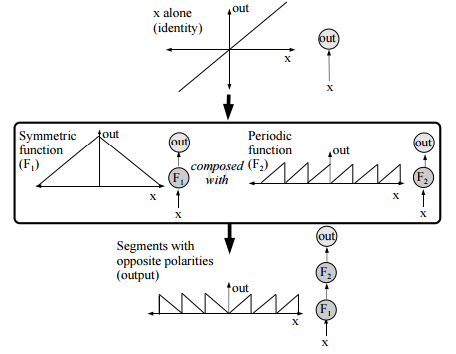
\includegraphics[width=.9\columnwidth]{cppn}
\caption{Composing two functions to obtain a single function which has multiple regularities \cite{Stanley2007}}
\label{fig:cppn}
\end{figure}

The evolution of CPPNs can be done using a method which is a variant of NEAT, CPPN-NEAT.
Specifically, where NEAT only operates with a network consisting of sigmoid-functions, CPPN-NEAT uses a range of different functions and chooses one at random when a new node is introduces into the network.
Furthermore, when determining if two individuals belong to the same species, the difference in which activation functions their hidden nodes use is taken into consideration.

CPPNs are of interest to our solution because of their symmetry producing properties.
%Stanley presented some experiments which used CPPNs to evolve two-dimensional images.
%The input to these networks were the x- and y-coordinates of the images, and the single output produced by the CPPN was used to colour the pixel at the given coordinate.

\subsection{Computer evolved tables}
\todo[inline]{Change this title?}
Evolutionary Algorithms have been used to develop similar solutions before. Examples of previous  applications are tables[See~figure~\ref{fig:hornby_tables}] where the optimisation parameters were height of the support structure, stability of the structure, and maximization of surface area.
\begin{figure}[ht]
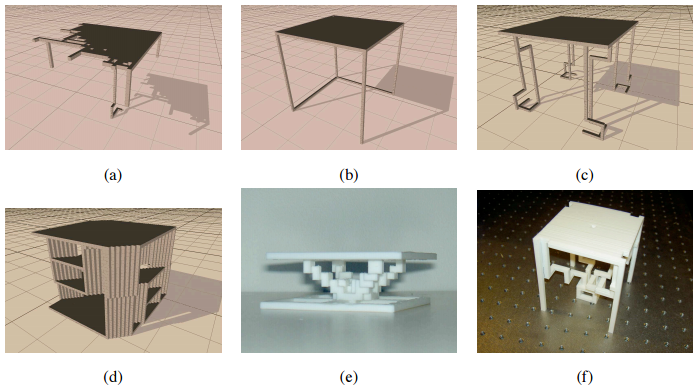
\includegraphics[scale=.6]{content/img/tables}
\caption{Image of Hornby tables\cite{paper:ev4}}
\label{fig:hornby_tables}
\end{figure}

While the evolution of tables has some similarities to seating they are inherently
different in the sense that maximized surface area might not be ideal for a
chair.
Neither would very high legs be optimal, since the physical attributes of humans
usually constrain us to some specific height range which is optimal for the
average persons seating comfort.

\subsection{Interactive Evolutionary Computation}
Takagi describes in his survey from 2001\cite{Takagi2001} how there are some \emph{``systems whose optimization indexes are difficult to specify''}\cite[p.~1275]{Takagi2001}.
For such systems, which include systems whose evaluation is aesthetic in nature, it is beneficial to use a human subject to evaluate the outcome of the Evolutionary Computation(EC).
This method is called Interactive Evolutionary Computation(IEC).

Some IEC is of interest to our solution, since we would like to guide the aesthetics of the designs our EC comes up with. 

\subsection{Evolving 3D objects with CPPNs}
In their paper from 2011 Klune and Lipson describe how they use CPPNs to evolve 3-dimensional objects\cite{Clune:2011:EOG:2078245.2078246}.
They describe how they encode the 3D objects with CPPNs by feeding the CPPN with three inputs, one each for the x-, y-, and z-coordinates of a 3D voxel space.
The single output of the CPPN for the given coordinates is checked against a threshold, and if it is above the threshold then the voxel in those coordinates is considered full, otherwise it is considered empty\cite[p.~5]{Clune:2011:EOG:2078245.2078246}.
They combine this encoding with IEC to evolve symmetrical 3D images, see figure~\ref{fig:3dobjects}.
\begin{figure}[ht]
\centering
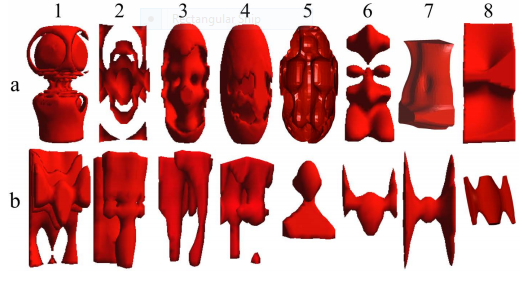
\includegraphics[width=.9\columnwidth]{3d_cppn}
\caption{Examples of the 3D images presented in \cite{Clune:2011:EOG:2078245.2078246}}
\label{fig:3dobjects}
\end{figure}


\section{Evolving chairs using NEAT}
To solve a problem using genetic algorithms, we need an encoding
consisting of a genotype, phenotype, and a mapping from genotype to phenotype.

Encodings can generally be divided into two categories; direct and generative
(or indirect). Generative encodings have several properties that lend themselves
well to our problem domain. By using a genotype encoding that \emph{generates}
the phenotype, a single sub-structure in the genome can encode several similar
sub-structures in the phenome. This makes it significantly easier to evolve
individuals that have symmetry or repetition, but with variation --- such as
chairs! While the Hornby study\cite{paper:ev4} uses Lindenmayer
systems\cite{Hornby2003}, we thought it would be interesting to try a
neuroevolutionary approach.

\subsection{Genetic Encoding}
As suggested by Stanley\cite{Stanley2007}, and as Clune and
Lipson\cite{Clune:2011:EOG:2078245.2078246} does, we consider the evolved CPPNs
to be a description of our phenotype, and query them with 3 Cartesian
coordinates, representing a point in 3d space. The output of the network then
determines the absence or presence of a voxel in that point, and hence whether
that point will be part of the chair's design. A voxel is present in a point if
the network outputs a vale larger than or equal to $0.5$ for that point.

This gives us a binary utility matrix representing a chair. To be able to render
and simulate physical experiments on it, we use the grassfire tranform, first
introduced by Harry Blum\cite{blum67}, to find a single connected component (If
there is more than one, we take the largest and discard the rest). We then
"hollow out" the chair --- we remove all voxels that are completely surrounded by
voxels. This is primarily to avoid representing them in the physical simulation,
which is computationally expensive.

\subsection{Evaluation}
The evaluation(fitness) function determines the value of each individual, in
each generation of the evolutionary experiment. For our fitness function we
considered the use of several static analysis terms, physical experiments, and
an interactive term.

For the static term, we considered analysis of sitting-surface area and angle,
but ended up relying on the physical simulation for this definition of
"chairdness" instead. The only static term we used in the end is the number of
voxels a chair consists of, corresponding to a measure of material cost.

for the physical simulation, we wanted to measure stability, as well as
viability as an object on which people can sit. In initial phases of the
project, we performed the experiment by dropping a sphere on the chair, and then
measuring the resulting rotation of the chair, the horizontal movement of the
sphere, and the height in which the sphere came to rest. In later stages, we
came to perform a similar experiment, but with a human rag doll. The rag doll
gave us the same information as the sphere, but with added opportunity to
measure a term for posture, by taking the vertical distance between the head and
hips.

The interactive term is used only conditionally. After evolving generations
without interaction (we have experimented with one, tens and hundredths of
generations between interaction), the user is allowed (but not forced) to select
a single individual out of the ten best. Selected individuals are then
remembered between generations, and their fitnesses artificially heightened,
with a decay over time.

For a phenome $p$, we concretely use the fitness function $F(P)$:
$$F(p) = -(|V| + R_c + E_{\Delta} + E_{rest} + E_{posture} + I)$$

Where $|V|$ is the number of voxels, approximating the material cost of the
chair, $R_c$ is linear in 
\subsection{Technologies (?)}

A solution using the Unity3D\cite{web:unity} game engine has been built. This has been done by building on a collegues work\cite{web:unityneat} with evolutionary algorithms, particularly a project porting SharpNeat\cite{web:sharpneat} to the Unity game engine.
While this is not directly applicable to our solution it supplied us with a framework for setting up evolutionary algorithms.
    
\textbf{Unity} was an arbitrary choice. We could just as easily have chosen any other game engine which provided the same components - particularly physics and rendering. However, Unity is used by thousands of people worldwide and has a lot of support provided by its active community which really works in favor of the engine.


\section{Results}
Several experiments were performed using the evaluation function mentioned in 
section \ref{sec:evaluation}. 

Initially the experiments were carried out without the interactive term, $I$,
and without regard for the mass of the individuals produced by the EC. This
meant that the physical part of the evaluation, where Ethan was dropped on the
individuals, resulted in the terms, $E_\Delta$, $E_{rest}$, and
$E_{posture}$ all being roughly equal. This happened because the higher mass of
Ethan would always result in the individuals being rotated and Ethan dropping
on the floor. This left only the $|V|$ and $R_c$ terms, and the EC ultimately
optimized towards a minimal voxel count which would not rotate when Ethan was
dropped, see figure~\ref{fig:flat_object}.

\begin{figure}[ht]
%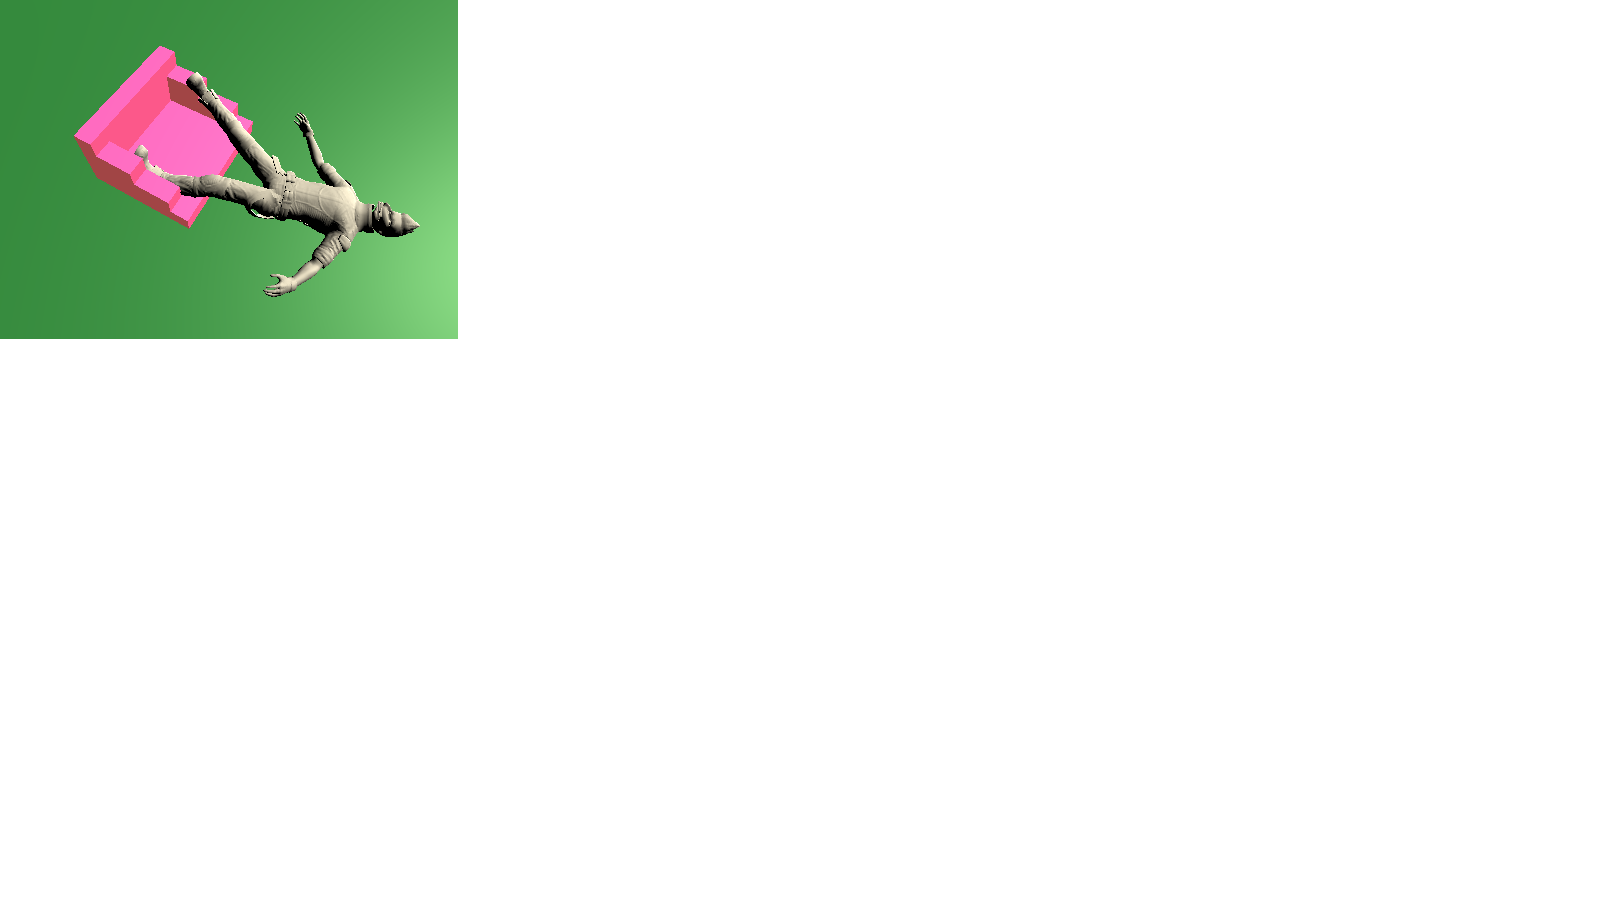
\includegraphics[width=.9\columnwidth]{footstool}
\missingfigure{Pretty picture of flat mat goes here.}
\caption{The evolved object, pink, is simply a flat structure, such that it 
does not rotate when Ethan is dropped on it, and has minimal voxel count.}
\label{fig:flat_object}
\end{figure}

Adding the interactive term, $I$, did not improve significantly on the above
results. While the selected individual would persist through several
generations, the other best performing individuals would still optimize towards
the aforementioned flat structure, see figure~\ref{fig:selection}.
\begin{figure}[ht]
\centering
\subfloat[]{
	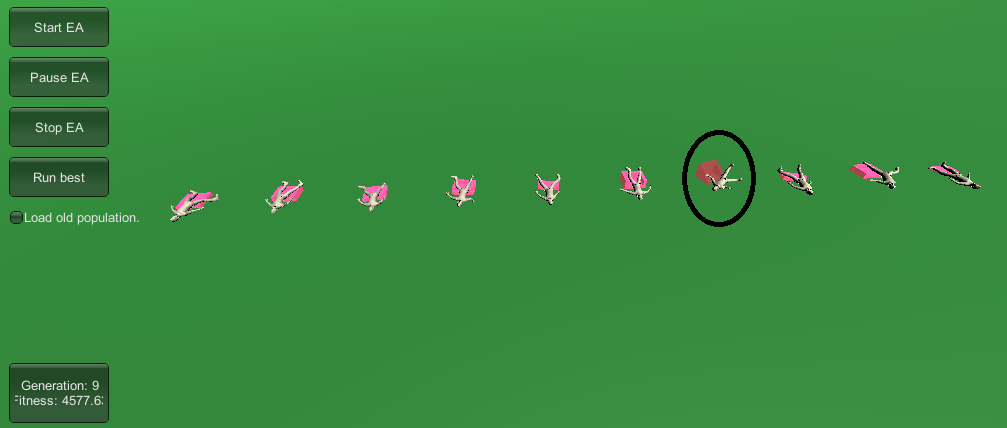
\includegraphics[width=.9\columnwidth]{selection}
}
\hfil
\subfloat[]{
	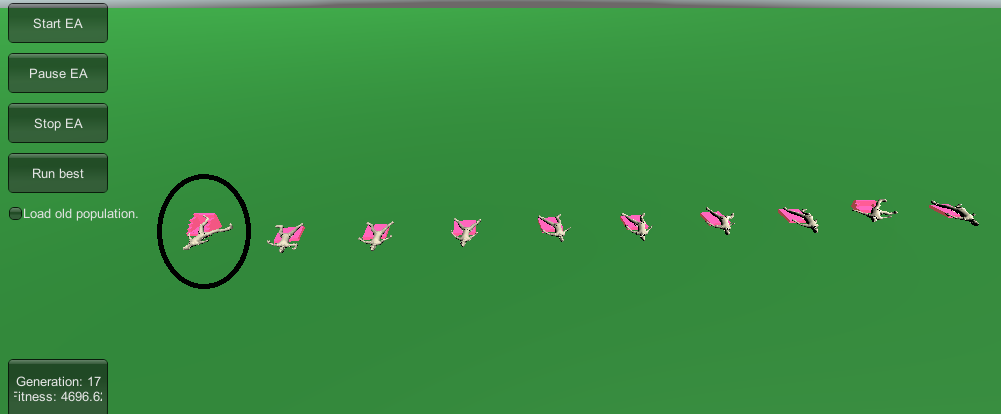
\includegraphics[width=.9\columnwidth]{selection2}
}
\caption{Example showing how the selected individual, encircled in (a), 
persists 8 generations later, encircled in (b).}
\label{fig:selection}
\end{figure}

Further experiments were conducted, where the mass of the individuals was
adjusted according to their voxel count. In these experiments the EC ended up
producing some individuals which were not just flat objects. Rather it 
produced individuals as boxes on which Ethan could rest in a height such that
the term $E_{rest}$ was minimized.
\section{Discussion}
While our results are interesting in their own right, it is always prudent to 
consider what might have been done differently in order to obtain other results.
\todo[inline]{more/better introduction}

\subsection{Incremental Evolution}
An approach to be considered is that of incremental evolution. Incremental
evolution would have allowed us to focus on a subset of desired properties ,
such as the desired height, or stability. Once a population had been evolved
which fulfilled the desired properties, the fitness function could be modified
to add another property. 

Using this approach it is plausible that we would have gotten better results,
as the individuals would not have to consider e.g. Ethan's posture, before they
had evolved to an appropriate height.

\subsection{Simulation Performance}
Our experiments suffer from the computational cost of simulating physical
experiments. To compensate for the time it takes to run these experiments, we
run experiments for only a few hundredths of generations, or with small
population sizes. This does not allow NEAT enough time, in the case of few 
generations, or lebensraum, in the case of small populations, to properly work.

As mentioned in section \ref{sec:results} our population size was 50 for the 
experiments which only ran for a couple of hundred generations, and 10 when we 
wanted the experiments to run for more generations.
Given more time we would have liked to tweak the NEAT parameters, such as
complexification and speciation, and not only the evaluation function.

\subsection{Rag Doll - (Ethan)}
While the idea to use a rag doll as part of the evaluation to evaluate the 
"chairness" of the individuals is novel, we realised too late that the rag doll 
we used in our simulations was not as flexible as first assumed.

Ethan did not bend in his hips and knees, resulting in him not being able to 
actually sit down. This helps explain why the individuals which tried to 
minimize the $E_{posture}$ term would evolve into shapes as seen on
figures~\ref{fig:metro_stand}~\&~\ref{fig:chair_legs}, as these individuals 
show features which help Ethan stand upright.

It would be nice to do some more experiments where Ethan's flexibility more
closely resembled that of a human.

\subsection{Interactive Evolutionary Computation}
Our use of IEC differs from that used by Clune and
Lipson\cite{Clune:2011:EOG:2078245.2078246}, in that we only prompt the user
for input every few generations. In most of our experiments this was roughly
every tenth generations. It would be interesting to see what would happen if we
instead had prompted the user every generation. 

It would also be interesting to try and combine the above mentioned approach
with that of incremental evolution. First one could use only human evaluation
to produce a population of individuals with interesting shapes. Then apply the
static physical evaluation to evolve the desired physical properties, or vice
versa.



% Computer Society journal (but not conference!) papers do something unusual
% with the very first section heading (almost always called "Introduction").
% They place it ABOVE the main text! IEEEtran.cls does not automatically do
% this for you, but you can achieve this effect with the provided
% \IEEEraisesectionheading{} command. Note the need to keep any \label that
% is to refer to the section immediately after \section in the above as
% \IEEEraisesectionheading puts \section within a raised box.

% An example of a floating figure using the graphicx package.
% Note that \label must occur AFTER (or within) \caption.
% For figures, \caption should occur after the \includegraphics.
% Note that IEEEtran v1.7 and later has special internal code that
% is designed to preserve the operation of \label within \caption
% even when the captionsoff option is in effect. However, because
% of issues like this, it may be the safest practice to put all your
% \label just after \caption rather than within \caption{}.
%
% Reminder: the "draftcls" or "draftclsnofoot", not "draft", class
% option should be used if it is desired that the figures are to be
% displayed while in draft mode.
%
%\begin{figure}[!t]
%\centering
%\includegraphics[width=2.5in]{myfigure}
% where an .eps filename suffix will be assumed under latex, 
% and a .pdf suffix will be assumed for pdflatex; or what has been declared
% via \DeclareGraphicsExtensions.
%\caption{Simulation results for the network.}
%\label{fig_sim}
%\end{figure}

% Note that IEEE typically puts floats only at the top, even when this
% results in a large percentage of a column being occupied by floats.
% However, the Computer Society has been known to put floats at the bottom.


% An example of a double column floating figure using two subfigures.
% (The subfig.sty package must be loaded for this to work.)
% The subfigure \label commands are set within each subfloat command,
% and the \label for the overall figure must come after \caption.
% \hfil is used as a separator to get equal spacing.
% Watch out that the combined width of all the subfigures on a 
% line do not exceed the text width or a line break will occur.
%
%\begin{figure*}[!t]
%\centering
%\subfloat[Case I]{\includegraphics[width=2.5in]{box}%
%\label{fig_first_case}}
%\hfil
%\subfloat[Case II]{\includegraphics[width=2.5in]{box}%
%\label{fig_second_case}}
%\caption{Simulation results for the network.}
%\label{fig_sim}
%\end{figure*}
%
% Note that often IEEE papers with subfigures do not employ subfigure
% captions (using the optional argument to \subfloat[]), but instead will
% reference/describe all of them (a), (b), etc., within the main caption.
% Be aware that for subfig.sty to generate the (a), (b), etc., subfigure
% labels, the optional argument to \subfloat must be present. If a
% subcaption is not desired, just leave its contents blank,
% e.g., \subfloat[].


% An example of a floating table. Note that, for IEEE style tables, the
% \caption command should come BEFORE the table and, given that table
% captions serve much like titles, are usually capitalized except for words
% such as a, an, and, as, at, but, by, for, in, nor, of, on, or, the, to
% and up, which are usually not capitalized unless they are the first or
% last word of the caption. Table text will default to \footnotesize as
% IEEE normally uses this smaller font for tables.
% The \label must come after \caption as always.
%
%\begin{table}[!t]
%% increase table row spacing, adjust to taste
%\renewcommand{\arraystretch}{1.3}
% if using array.sty, it might be a good idea to tweak the value of
% \extrarowheight as needed to properly center the text within the cells
%\caption{An Example of a Table}
%\label{table_example}
%\centering
%% Some packages, such as MDW tools, offer better commands for making tables
%% than the plain LaTeX2e tabular which is used here.
%\begin{tabular}{|c||c|}
%\hline
%One & Two\\
%\hline
%Three & Four\\
%\hline
%\end{tabular}
%\end{table}

%\pagebreak

% use section* for acknowledgment
\ifCLASSOPTIONcompsoc
  % The Computer Society usually uses the plural form
  \section*{Acknowledgments}
\else
  % regular IEEE prefers the singular form
  \section*{Acknowledgment}
\fi


The authors would like to thank Sebastian Risi, ITU, Andres Faina, ITU and Laura Beloff, ITU.

% Can use something like this to put references on a page
% by themselves when using endfloat and the captionsoff option.
\ifCLASSOPTIONcaptionsoff
  \newpage
\fi



% trigger a \newpage just before the given reference
% number - used to balance the columns on the last page
% adjust value as needed - may need to be readjusted if
% the document is modified later
%\IEEEtriggeratref{8}
% The "triggered" command can be changed if desired:
%\IEEEtriggercmd{\enlargethispage{-5in}}

% references section

% can use a bibliography generated by BibTeX as a .bbl file
% BibTeX documentation can be easily obtained at:
% http://www.ctan.org/tex-archive/biblio/bibtex/contrib/doc/
% The IEEEtran BibTeX style support page is at:
% http://www.michaelshell.org/tex/ieeetran/bibtex/
\bibliographystyle{IEEEtran}
% argument is your BibTeX string definitions and bibliography database(s)
\bibliography{bibliography}
%
% <OR> manually copy in the resultant .bbl file
% set second argument of \begin to the number of references
% (used to reserve space for the reference number labels box)

%\vfill

% Can be used to pull up biographies so that the bottom of the last one
% is flush with the other column.
%\enlargethispage{-5in}



% that's all folks
\end{document}


